% Licensed under the Creative Commons Attribution Share Alike 4.0 International.
% See the LICENSE file in the repository root for full license text.

\section{实验:CMake 的基本工作流程\label{sec:experiment-3}}

图 \ref{fig:cmake-gui-2} 中,需要在最上面的编辑框中填写源代码所在目录。CMake 程序并不直接帮助你搜集该目录下源代码的信息,而是根据目录下名为 \lstinline[language={}]{CMakeLists.txt} 的文本文件进行工作。所以,学习 CMake 实际上是指学习编写 \lstinline[language={}]{CMakeLists.txt} 文件,我们将从下一章开始讨论。本实验中,我们将聚焦 CMake 程序的使用方法。

\subsection*{实验步骤}

\begin{enumerate}
	\item 新建空白 CMakeLists 文件。在工作目录下新建文件夹,并在其中新建一个文本文件,命名为 \lstinline[language={}]{CMakeLists.txt}。

	\begin{remark}
		没错,尽管其他教程可能已经开始教你如何建立一个最小工程了,但我们在两章后才做这件事。现在的 \lstinline[language={}]{CMakeLists.txt} 就是一个空文件。
	\end{remark}

	\item 在 cmake-gui 中打开新建的文件夹。\label{item:exp-3-2}

	从开始菜单打开 cmake-gui,点击“Brouse Source...”按钮,选择刚才新建的文件夹。再将图 \ref{fig:cmake-gui-2} 中“生成文件的目录”设定为工作目录下的另一个文件夹(通常以 \lstinline[language={}]{build} 开头命名),如图 \ref{fig:empty-cmake-1} 所示。

	\begin{figure}[H]
		\centering
		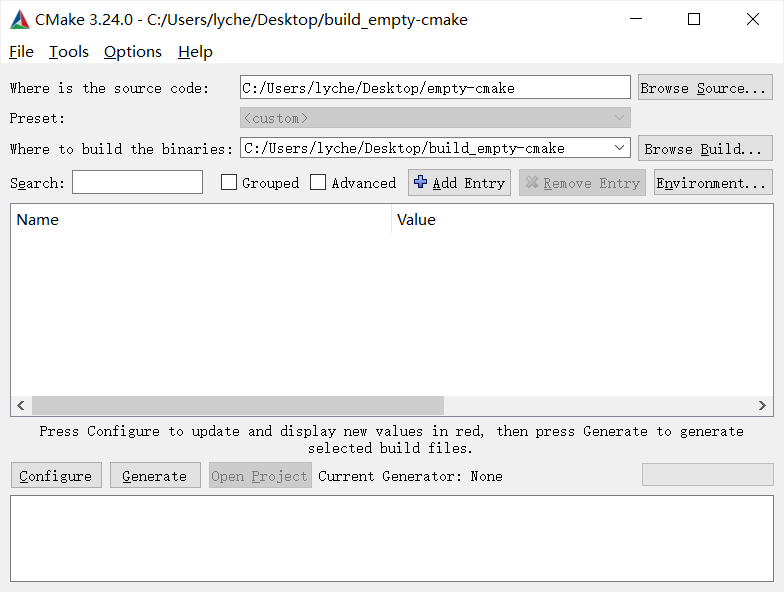
\includegraphics[width=0.65\linewidth]{assets/empty-cmake-1}
		\caption{填写源代码所在目录和生成文件目录的示例。}
		\label{fig:empty-cmake-1}
	\end{figure}

	\item 配置项目。\label{item:exp-3-3}

	点击图 \ref{fig:cmake-gui-1} 中的“Configure”按钮,弹出对话框提示生成文件的目录不存在,需要创建文件夹(图 \ref{fig:empty-cmake-2}),点击“Yes”。

	\begin{figure}[H]
		\centering
		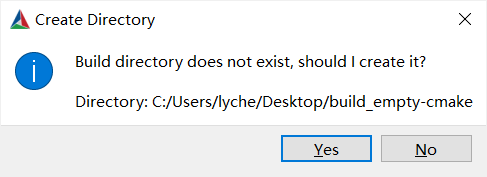
\includegraphics[width=0.35\linewidth]{assets/empty-cmake-2}
		\caption{提示创建生成目录文件夹的对话框。}
		\label{fig:empty-cmake-2}
	\end{figure}

	随后弹出图 \ref{fig:empty-cmake-3} 所示的对话框。目前我们不研究它,直接点击“完成”(“Finish”)\footnote{此处要求已安装图 \ref{fig:empty-cmake-3} 中显示的 Visual Studio 2022。如果你没有安装,请点击该下拉列表框,选择计算机中已安装的编译器。之后的内容以 Visual Studio 2022 为例。}。

	\begin{figure}[H]
		\centering
		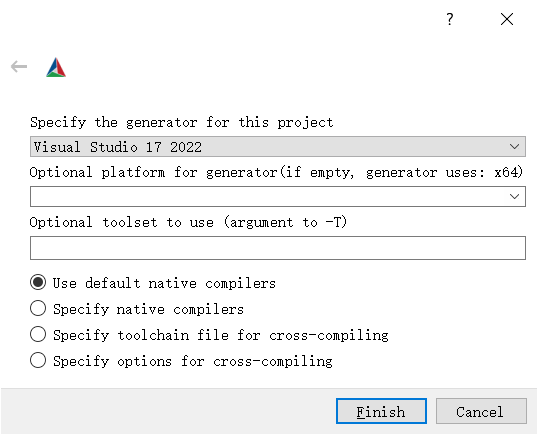
\includegraphics[width=0.4\linewidth]{assets/empty-cmake-3}
		\caption{一个对话框,目前我们不研究它。}
		\label{fig:empty-cmake-3}
	\end{figure}

	然后可以观察到图 \ref{fig:empty-cmake-4} 所示的主窗口。

	\begin{figure}[H]
		\centering
		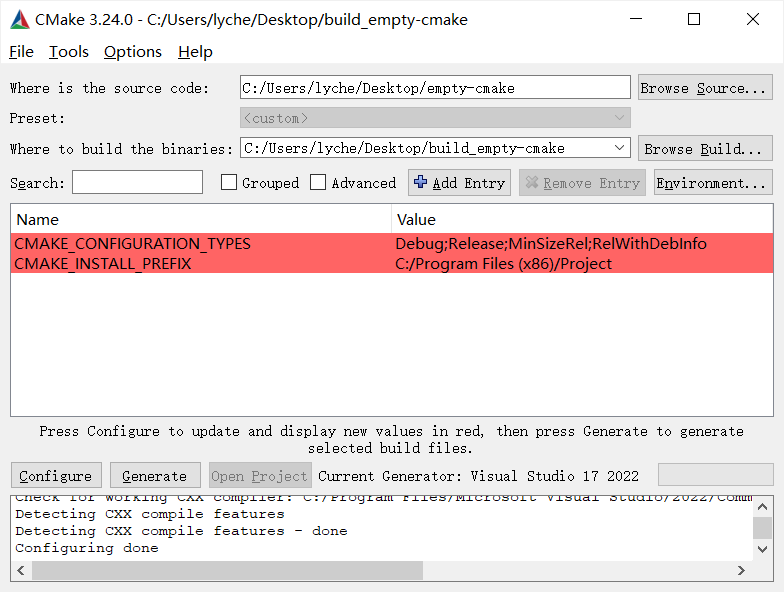
\includegraphics[width=0.7\linewidth]{assets/empty-cmake-4}
		\caption{配置项目后的 cmake-gui 主窗口。}
		\label{fig:empty-cmake-4}
	\end{figure}

	前往查看源代码所在目录和生成文件的目录。发现源代码所在目录下的文件并未发生变化,而生成文件的目录下出现了图 \ref{fig:empty-cmake-5} 所示的文件。

	\begin{figure}[H]
		\centering
		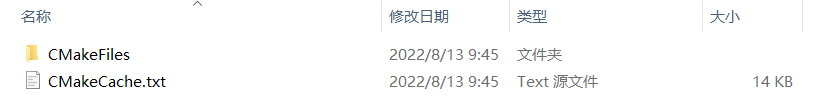
\includegraphics[width=0.9\linewidth]{assets/empty-cmake-5}
		\caption{配置项目后生成的文件。}
		\label{fig:empty-cmake-5}
	\end{figure}

	\item 生成项目。\label{item:exp-3-4}

	点击图 \ref{fig:cmake-gui-1} 中的“Generate”按钮,观察到 cmake-gui 的日志文本框中直接显示“Generating done”。

	前往查看源代码所在目录和生成文件的目录。发现源代码所在目录下的文件仍未发生变化,而生成文件的目录下额外出现了 Visual Studio 项目文件,如图 \ref{fig:empty-cmake-6} 所示。

	\begin{figure}[H]
		\centering
		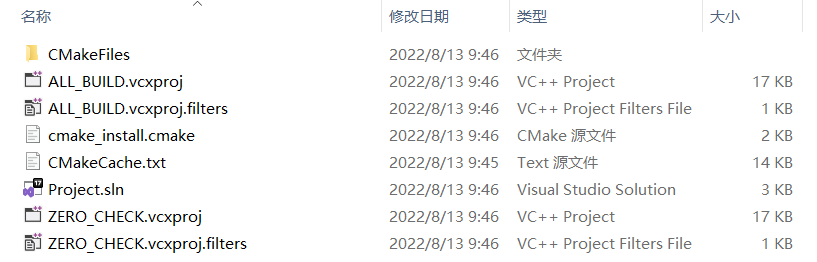
\includegraphics[width=0.9\linewidth]{assets/empty-cmake-6}
		\caption{生成项目后生成的文件。}
		\label{fig:empty-cmake-6}
	\end{figure}
\end{enumerate}

\subsection*{讨论}

\begin{enumerate}
	\item CMake 的基本工作流程总结。

	CMake 的工作可以分为\emph{配置项目(configure)}和\emph{生成项目(generate)}这两个步骤。具体而言:

	\begin{itemize}
		\item 配置项目的作用是检测编译器支持的\emph{特性(feature)}(见图 \ref{fig:empty-cmake-4} 中的日志文本框)、更新缓存变量文件 \lstinline[language={}]{CMakeCache.txt}。概括地说,\textbf{它的功能是收集 CMake 自身所需要的全部信息}。

		\item 生成项目的作用是根据 CMake 收集的信息\textbf{生成项目工程文件},例如图 \ref{fig:empty-cmake-6} 中的 Visual Studio 解决方案文件 \lstinline[language={}]{Project.sln}。除此之外,也可以指定 CMake 生成 makefile 文件,我们将在之后介绍相关内容。 % TODO: 指定章节、概括得更具体。
	\end{itemize}

	可以看出,CMake 本身并不参与 C++ 程序的\emph{生成(build)},\textbf{它的主要功能是生成用户需要的项目工程文件}。因此,CMake 跨平台的能力来自它对不同平台上不同编译器的广泛支持。只要你的计算机中安装有支持的编译器,CMake 就能通过你编写的 \lstinline[language={}]{CMakeLists.txt} 生成适合该编译器的文件,也就实现了一份源代码处处编译的愿景——当然,前提是你编写的 C++ 源代码本身跨平台且足够好,不会因为更换了编译器而编译失败。

	值得注意的是,配置项目和生成项目通常会合成一步,统称为\emph{配置项目(configure)}。图 \ref{fig:configure} 展示了各名词之间的关系。

	\begin{figure}[H]
		\centering
		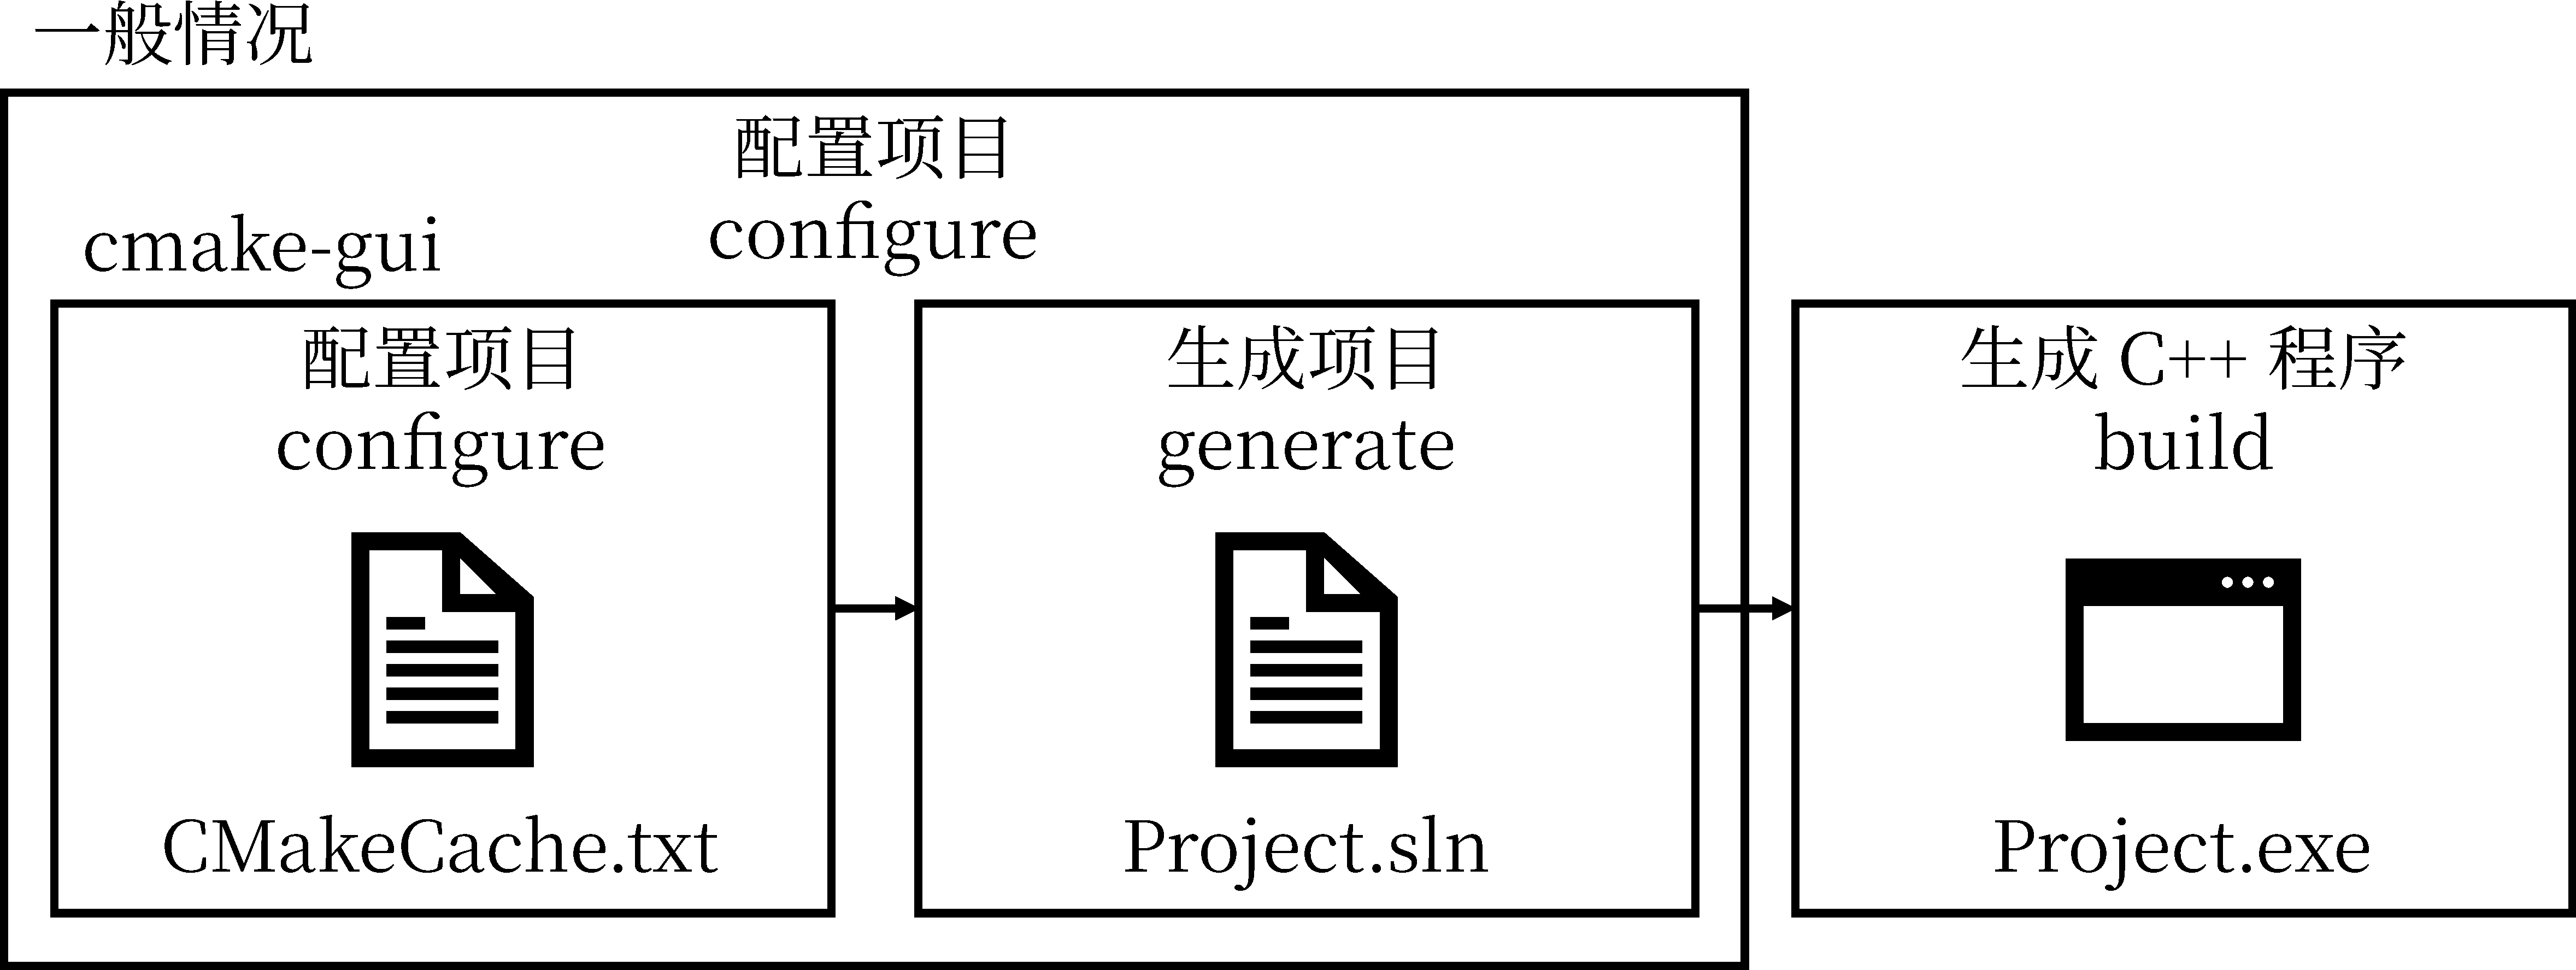
\includegraphics[scale=0.15]{assets/configure}
		\caption{配置项目(configure)、生成项目(generate)、生成(build)之间的关系。}
		\label{fig:configure}
	\end{figure}

	为了进一步降低开发难度,\textbf{还可以通过命令行让 CMake 帮助我们调用编译器或生成工具},所以可以认为图 \ref{fig:configure} 中的“生成 C++ 程序”也属于 CMake 的工作流程。

	\item \lstinline[language={}]{CMakeCache.txt}。

	在 cmake-gui 中点击配置项目后,用文本编辑器打开生成的 \lstinline[language={}]{CMakeCache.txt},部分内容如图 \ref{fig:cmake-cache} 所示。

	\begin{figure}[H]
		\centering
		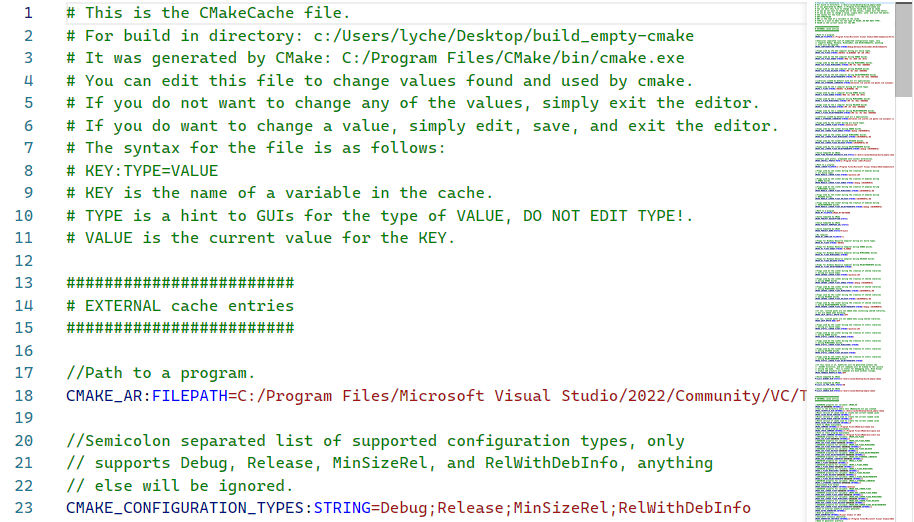
\includegraphics[width=0.8\linewidth]{assets/cmake-cache}
		\caption{\lstinline[language={}]{CMakeCache.txt} 内容节选。}
		\label{fig:cmake-cache}
	\end{figure}

	可以看到,\lstinline[language={}]{CMakeCache.txt} 中保存的\textbf{缓存变量是一系列的键值对},只有 \lstinline[language={}]{KEY:TYPE=VALUE} 一种语法。对比图 \ref{fig:empty-cmake-4} 和图 \ref{fig:cmake-cache},发现图 \ref{fig:empty-cmake-4} 中的缓存变量要少很多。要解决这一问题,只需点击 cmake-gui 中的 Advanced 复选框,就能在列表中显示所有的缓存变量了。

	\item 生成目录不要与源代码所在目录相同。

	第 \ref{item:exp-3-2} 步中,我们要求将生成文件的目录设定为工作目录下的另一个文件夹。如果令生成目录完全等于源代码所在目录,可以预见,步骤 \ref{item:exp-3-3} 和步骤 \ref{item:exp-3-4} 中生成的项目文件(图 \ref{fig:empty-cmake-6})将直接出现在源代码所在目录中,破坏我们的源代码结构,所以\textbf{一定不能把生成目录直接设定为源代码所在目录}。
	% TODO: 指定章节。
	之后我们可以编写 CMake 代码阻止生成目录与源代码目录完全相同的情况发生。

	通常,可以指定生成目录为源代码目录下的一个子文件夹,例如该实验中可以指定为 \lstinline[language={}]{~/Desktop/empty-cmake/build}。之所以我们在第 \ref{item:exp-3-2} 步把生成目录指定在了源代码目录的外面,是因为 CMakeLists 可以请求检索源代码目录下的\textbf{所有}文件。如果生成的文件出现在了源代码文件夹中,即使它们位于单独的文件夹中,也仍可能对 CMake 的文件检索造成影响。因此,\textbf{应当尽可能把生成目录指定在源代码所在目录外}。

\end{enumerate}
